%-----------------------------------------------------------------------------------------------
%		\COMPdataFormatManagement{} Design
%-----------------------------------------------------------------------------------------------

\section{\COMPdataFormatManagement{} Design}
\label{sec:COMPdataFormatsDesign}

In this section, the design of the component \COMPdataFormatManagement{} is described. Basic task of the component is to describe the structure of a container or metadata format in a way that is useful for parsing them generically.

% =======================================================================================================
\subsection{Format Comparison}%
\label{sec:FormatComparison}%

Before any real design decisions can be found, we have to look what the formats are that we try to generically describe with the \COMPdataFormatManagement{} component. The main source of this whole chapter is \cite{MC17}.

We fully focus on the following data formats here, ignoring any other possible formats as out of scope:
\begin{itemize}
\item Multimedia container formats: Ogg, QuickTime, MPEG Layer I Elementary Stream (for MP3), Matroska, RIFF
\item Metadata container formats: ID3v1 and ID3v1.1, ID3v2.2, ID3v2.3, ID3v2.4, VorbisComment, Lyrics3v1, Lyrics3v1, APEv1 and APEv2
\end{itemize}

As first introduction, we have to compare those formats according to their most important structural aspects. These aspects are as follows:
\begin{itemize}
\item Basic encoding they use: \textbf{Byte orders} and \textbf{character encodings} supported
\item Building blocks: What are the \textbf{containers} in this format? Are there other sub-structures? Can they be embedded in each other? Is there a hierarchical structure with arbitrary nesting? For metadata container formats, we call the elements actually holding the metadata \emph{attributes}, which is nothing else than a special case of a container.
\item Headers and Footers: Despite the payload, are there \textbf{headers} and/or \textbf{footers} in the containers or attributes? Are they fixed or variable size?
\item Lengths of containers: How is the \textbf{length of containers} or of their payload defined?
\item Lengths of attributes: How is the \textbf{length of attributes} for metadata container formats defined?
\item Padding: Does the format have some special way of supporting \textbf{padding}?
\end{itemize}

The following table provides all these properties for multimedia container formats, skipping attribute topics:

TODO Table for multimedia formats
tab:DFcompareMult

The following table compares these properties for the metadata container formats considered:

TODO Table for metadata formats
tab:DFcompareMeta

Note that ID3v2x is a very special format in multiple dimensions: It is incredibly overloaded with a lot of features you might never dare dream to use, say: over-designed. It offers e.g. support for encryption, grouping, compression of tags, embedded lyrics or audio guide codec data which basically contain spoken versions of the metadata stored and other things. On top of that, it has a strange conversion scheme called the \emph{unsynchronization scheme}. 

% =======================================================================================================
\subsection{The Container Metamodel}%
\label{sec:TheContainerMetamodel}%

In order to give a feasible model of the structure of a container format (which includes metadata container formats), a metamodel of the typical data structure of a container format is developed here. 

The metamodel is ultimately shown in the following figure, the corresponding design decisions will follow:

\begin{figure}[htbp]
\centering
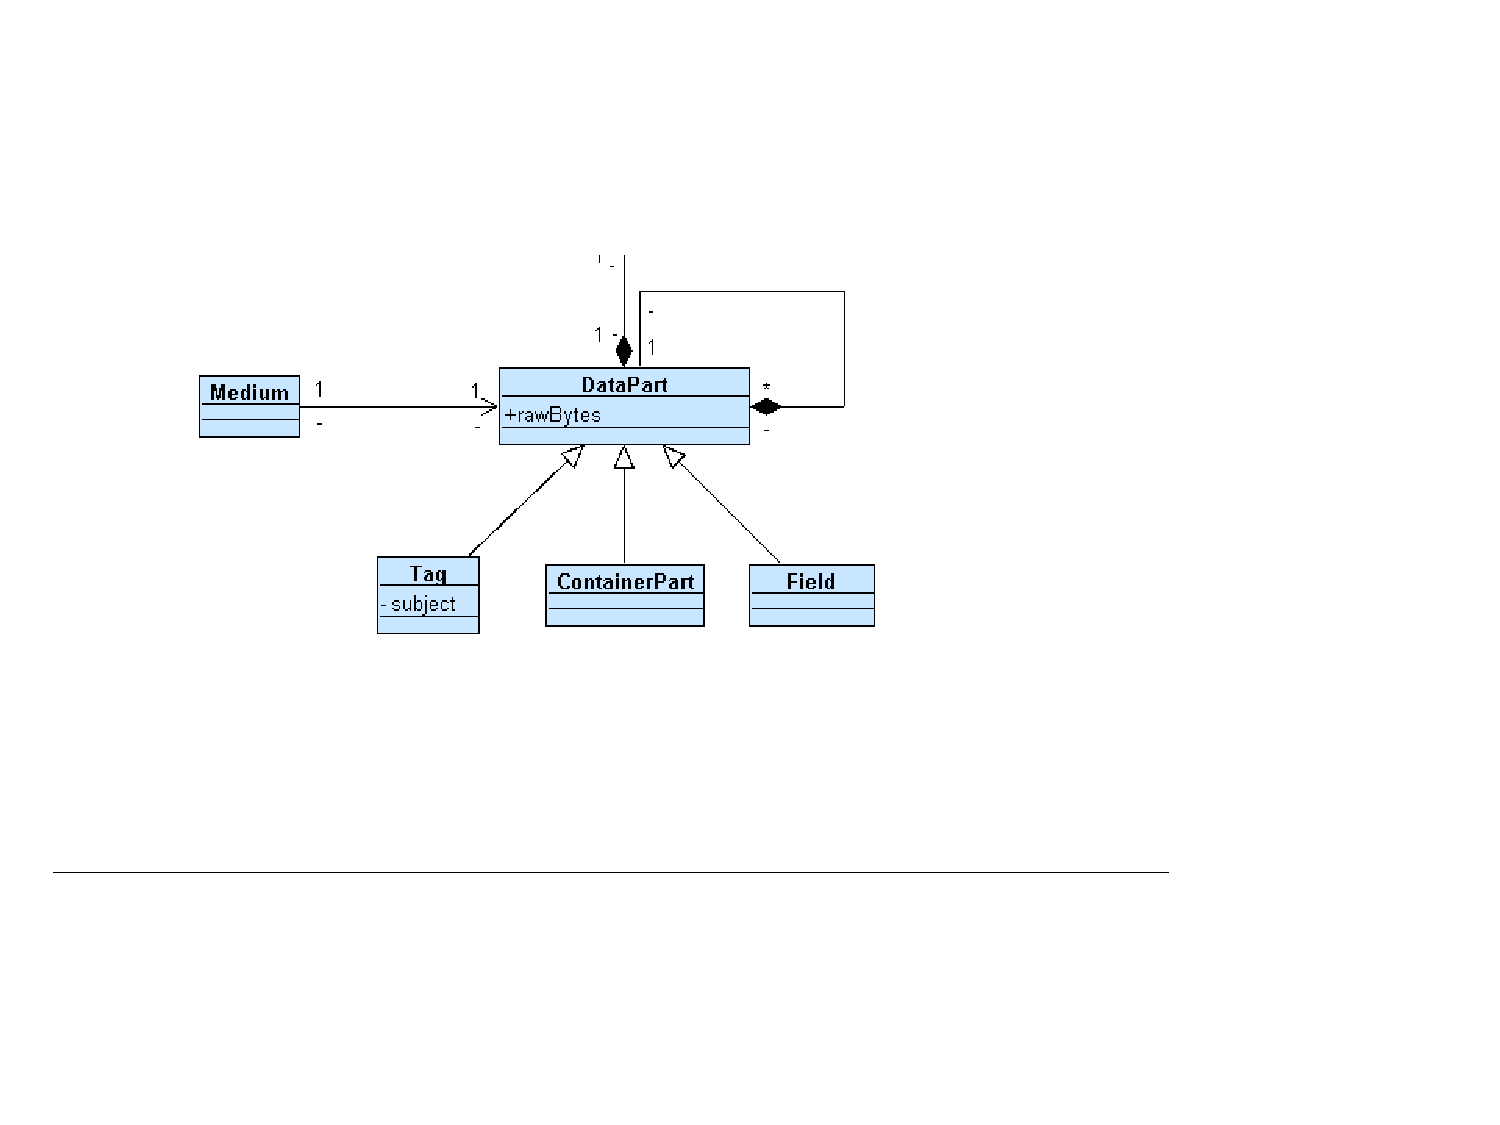
\includegraphics[width=1.00\linewidth]{figures/II_GeneralModel.pdf}
\caption{The container metamodel}
\label{fig:II_GeneralModel}
\end{figure}

%%%% DD --> %%%%
\DD{dd:500}
{% Title
Containers as basic top-level unit, containing nested containers
}
{% Short description
All data that can be processed by \LibName{} consists of containers. A container is a sequence of bytes with a specific structure belonging to exactly one container data format. However, consecutive containers might belong to different data formats.

In addition, a container - as the name suggests - contains other data. This data might be containers of the same format again. The nesting might be arbitrarily deep. A nested container is able to contain data of other formats. 
}
{% Rationale
Every format considered here has such basic building blocks, called differently in each format specification (atom, frame, page, element, item, tag etc.). The same file or media stream might consist of containers belonging to different formats. One example is an MP3 file with an ID3v2 tag. See also \cite{MC17}, part IV for more details.

Most of the supported data formats have some notion of nesting child containers (or, for metadata formats: attributes) within parent containers. Those child containers have either exactly the same stucture as the top-level containers, or they differ slightly. Some formats such as RIFF explicitly define specific containers that embed data belonging to other metadata formats. 
}
{% Disadvantages
No disadvantages known
}
%%%% <-- DD %%%%

How are these containers structured in detail?

%%%% DD --> %%%%
\DD{dd:501}
{% Title
A container consists of an optional \textbf{header}, \textbf{payload} and an optional \textbf{footer}
}
{% Short description
Every container - no matter which data format - follows the same basic structure: An optional header starts the containers byte sequence. Following this, there is a sequence of bytes called the payload. At the end of the container, there is an optional footer. A container must either have a header or a footer.
}
{% Rationale
Considering table \ref{tab:DFcompareMult} and \ref{tab:DFcompareMeta}, every container in every format has at least one header or one footer, including nested containers. Only ID3v23 as sole exception has a second, so-called extended header. To be discussed soon how this will be handled. We do not want to add additional complexity by having multiple headers or footers just because of this singular case. Modelling the middle part of a container as payload explicitly instead of just as list of sub-containers or fields makes sense because it allows to lazily read substructures, or entirely skip the payload.
}
{% Disadvantages
No disadvantages known
}
%%%% <-- DD %%%%

We saw that containers have a structure, and containers can live within other containers. But on the lowest level, there are leaf nodes, the fields:

%%%% DD --> %%%%
\DD{dd:502}
{% Title
Fields as the atomic unit of all byte sequences
}
{% Short description
\textbf{Field}s are the leaf nodes of the container metamodel: A field is a sequence of 1 to N consecutive bytes. A field has a \textbf{binary value} as well as an \textbf{interpreted value}, i.e. a human-understandable value with a specific meaning. We say that a field has a specific type, which basically describes the mapping between binary and interpreted value as well as the allowed values or format of a field.
}
{% Rationale
The term ``field'' is quite commonly used in binary data formats. It does not make sense to go down to individual byte or bit level. The smalles level of semantic in every binary or textual format is a field.
}
{% Disadvantages
No disadvantages known
}
%%%% <-- DD %%%%

Now towards headers and footers: Are they inherently different or basically the same? Fixed or variable size?

%%%% DD --> %%%%
\DD{dd:503}
{% Title
Headers and footers as sequences of fields are structurally identical
}
{% Short description
Headers and footers are sequences of fields, i.e. they must not nest a container. They are either variable or fixed-size. For ID3v2, the extended header can be seen as extending the mandatory ID3v2 header, i.e. the usual static header becomes a potentially larger, i.e. variable sized header. This eliminates the need to have multiple headers in the metamodel. For both header and footer, the same model class called FieldSequence is used.
}
{% Rationale
No data format specifies a header or footer nesting a container-like data structure, they all consist of plain fields. Despite the location (before or behind the payload), there is nothing really distinguishing headers or footers from a structural perspective. Thus the same model class can be used for both. However, there is no english term for that class that seems to clearly be a grouping term for headers and footers.
}
{% Disadvantages
No disadvantages known
}
%%%% <-- DD %%%%

So far, we just introduced containers, fields, headers, footers and payload. We learned that containers might embed other containers, while headers and footers must only consist of fields. But what about the structure of the payload of a container? Of course, if the headers and footers cannot embed child containers, they must hide within the payload. Is this the only possibility? Of course not:
%%%% DD --> %%%%
\DD{dd:504}
{% Title
Payload either solely consists of containers or fields
}
{% Short description
The payload of a container either fully consists of a sequence of child containers or of a sequence of fields, but never both.
}
{% Rationale
Ultimately, we must boil payload down of fields, or put otherwise: We cannot recurse indefinitely into sub-containers. So at last, there must be a final sequence of child containers having payloads solely consisting of fields. So it is clear that we have both cases. But what about the mixed case: Should we have containers in the model that have both child fields neighbouring child containers? In rare cases such as - again - ID3v2, it would be possible to think of having the frames as child containers of the tag, followed by the padding child field of the tag behind it. However, we avoid such complexities, but payload is either ContainerBasedPayload or FieldBasedPayload. See next design decision of how we handle the ID3v2 special case.
}
{% Disadvantages
No disadvantages known
}
%%%% <-- DD %%%%

How how to handle padding? If we look at the data format comparisons in \ref{tab:DFcompareMult} and \ref{tab:DFcompareMeta}, we see that padding is just a special case in ID3v2 and MP3. All other format solve it ``more naturally'' by embedding it in special child container. ID3v2 just adds some nullbytes at the end of the tag payload behind the frames. How to model this? There are basically three possibilities:
\begin{itemize}
\item The padding is a part of the payload, basically a field. This seems most intuitive, but is already excluded by the previous design decision, because then we would need to support mixed payloads, consisting both of child containers and fields.
\item The padding is part of the payload, but considered as a very special child container.
\item The padding is an optional part of the tag footer.
\end{itemize}

Based on these alternatives, we can really only decide the following:
%%%% DD --> %%%%
\DD{dd:505}
{% Title
Padding in ID3v2 is modeles as very special child container of the tag
}
{% Short description
Padding in ID3v2 is modeled as very special child container of the tag, where the header is the first null byte, and all follow-up bytes form the payload. 
}
{% Rationale
Modeling it as child field of the payload is not possible as it would contradict \DesLink{dd:504}. Modeling as part of the footer would be odd, as not every version of ID3v2 defines a footer at all, and we would have a variable sized footer optionally starting with an arbitrary number of nullbytes, which would not be very intuitive from a library users perspective, too.
}
{% Disadvantages
The only disadvantage possibly to be identified that there could be padding just consisting of a single byte. This would mean we'd have a container with just a header, but an empty payload, which actually is quite degenerate.
}
%%%% <-- DD %%%%


%###############################################################################################
%###############################################################################################
%
%		File end
%
%###############################################################################################
%###############################################################################################